\chapter{Results}
\let\cleardoublepage\clearpage 

General characteristics of the study population are displayed in Table \ref{pop}.
\tabularnewline
\tabularnewline

\begin{table}[bp]
\centering
\begin{tabular}{llllll}
\hline
                   & All Participants &  & Cases       &  & Controls    \\ \hline
n                  & 9663             &  & 5831        &  & 3832        \\
Age$^1$ (years)       & 62.8 $\pm$ 12.3      &  & 56.2 $\pm$ 10.1 &  & 73.0 $\pm$ 7.4  \\
Smoke Current (\%) & 29.6             &  & 36          &  & 20          \\
Male (\%)          & 65.3             &  & 76.7        &  & 47.9        \\
Obese $^2$ (\%)       & 29               &  & 35.1        &  & 19.7        \\
BMI (kg/$m^2$)        & 28.1 $\pm$ 5.3       &  & 28.9 $\pm$ 5.3  &  & 26.7 $\pm$ 4.9  \\
TG $^3$ (mmol/L)      & 1.46 $\pm$ 1.47      &  & 1.66 $\pm$ 1.70 &  & 1.18 $\pm$ 0.99 \\
HDLc$^3$ (mmol/L)     & 1.27 $\pm$ 0.44      &  & 1.13 $\pm$ 0.39 &  & 1.46 $\pm$ 0.44 \\
LDLc$^3$ (mmol/L)     & 3.29 $\pm$ 1.08      &  & 3.18 $\pm$ 1.17 &  & 3.43 $\pm$ 0.93 \\ \hline
\end{tabular}
\caption[General Population descriptions.]{General Population description. All values are expressed as mean $\pm$ one standard deviation unless otherwise noted. $^1$  Age represents age at consent for controls and age at diagnosis for cases
 $^2$ Obesity is defined as having a BMI of greater or equal to 30 kg/m2 at time of collection $^3$T G (triglyceride), LDLc (low density lipoprotein cholesterol), HDLc (high density lipoprotein cholesterol).}
\label{pop}
\end{table}


\section{Traditional Risk Score}

The traditional risk score was significantly ($P < 2.2 \times 10^{16}$) associated with case/control status in all cohorts when adjusted for principal components to control for population stratification. \citep{Price2006,Zhang2013}. On average, scores between cases and control differed by $5.06 \times 10^{-4} \pm 1.73 \times 10^{-4}$. Full distributions of the score dependent on case control status are presented in Supplementary Figure 4.1. $\hat{S}_{TRS}$ predicted CAD status better than chance in all cohorts. Area under the receiver operator characteristic curve was calculated for each model and meta-analysed. The resulting AUC $\pm$ 95\% confidence intervals are displayed in Figure \ref{trs_meta}.

\begin{figure}[h]
\label{trs_meta}
\centering
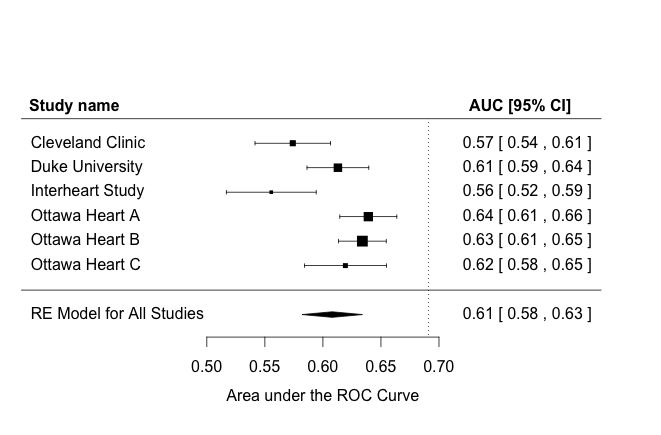
\includegraphics[width=0.8\textwidth]{Figures/trs_meta.png}
\caption[Random effects meta analysis of AUC ROC from six cohorts.]{\textbf{Random effects meta analysis of AUC ROC from six cohorts.} Logistic regression models were constructed with $\hat{S}_{TRS}$ and the first two principal components adjusting for population stratification were used to predict \ac{CAD}. Various thresholds for false positives and true positives were used to construct \ac{ROC} curves. Area under these curves were estimated along with error. The associated effects were analyzed assuming cohorts were random effects and an overall effect was derived.}
\end{figure}

Logistic regression was used to predict observations following the model. Summary statistics from the models employed are displayed in Table \ref{trs}

$$ CAD = X_0 + \hat{\beta}_1 \hat{S}_{TRS} + \hat{\beta}_2 PC_1 + \hat{\beta}_3 PC_3 + \epsilon $$

\begin{table}[H]
\centering

\begin{tabular}{llllll}
\hline
Cohort           & OR        & SE       & $R^2$      & AIC      & AUC       \\ \hline
Cleveland Clinic & 153.89908 & 36.42776 & 0.01621871 & 1877.724 & 0.5740551 \\
Duke University  & 255.78537 & 33.44304 & 0.04713465 & 2335.567 & 0.6129263 \\
Interheart       & 83.95637  & 46.45943 & 0.01695232 & 1172.994 & 0.5554871 \\
OHGS A2          & 310.49752 & 34.52749 & 0.07650691 & 2558.277 & 0.6391285 \\
OHGS B2          & 259.59352 & 24.94511 & 0.07425403 & 3681.768 & 0.6339916 \\
OHGS C2          & 276.96733 & 45.92012 & 0.05491302 & 1318.919 & 0.6193695 \\ \hline
\end{tabular}
\caption[Summary statistics from Logistic association model for $\hat{S}_{TRS}$.]{\textbf{Summary statistics from Logistic association model.} $\hat{S}_{TRS}$ along with the first two principal components to adjust for population stratification were used to predict \ac{CAD}. OR corresponds to the odds ratio of $\hat{S}_{TRS}$ along with its standard error (SE). $R^2$ corresponds to NagelKerke's Pseudo-$R^2$, while AIC corresponds to Akaike Information Criterion, a measure of model fit. AUC corresponds to the area under the \ac{ROC} curve as derived in the pROC package in R.}
\label{trs}
\end{table}

An \ac{AUC} $\geq 0.5$ indicates that the model predicts CAD better than chance. The overall random effects meta analyzed \ac{AUC} was 0.61 $\pm 0.03$ for $\hat{S}_{TRS}$, with an average NagelKerke's Pseudo-$R^2$ of $0.047$. Interheart was the worst fit model, with NagelKerke's Pseudo-$R^2 = 0.017$ and \ac{AUC} $= 0.555$, barely predicting above chance. This is in contrast to the OHGS cohorts, which consistently fit better than Cleveland Clinic, Duke, or Interheart. As increasing the number of \acs{SNP} in the score will always increase the fit of the model, we compare the 202 FDR significant loci to randomly selected loci in 1000 bootstraps in Figure \ref{b2_perm}. 

The score remains significantly associated when adjusted for individual's sex, a known cardiovascular risk factor. The predictive accuracy of the model significantly increases after inclusion of sex, as would be expected. The random effects meta analysis \ac{AUC} for all six cohorts becomes $0.69[0.62, 0.76]$. 

In \ac{OHGS} B2, sex significantly ($P = 0.00226$) interacts with the effect of the risk score. This shows that sex modulates the effect of genetics in this cohort. The remainder of the cohorts do not interact.


\begin{figure}[H]
\centering
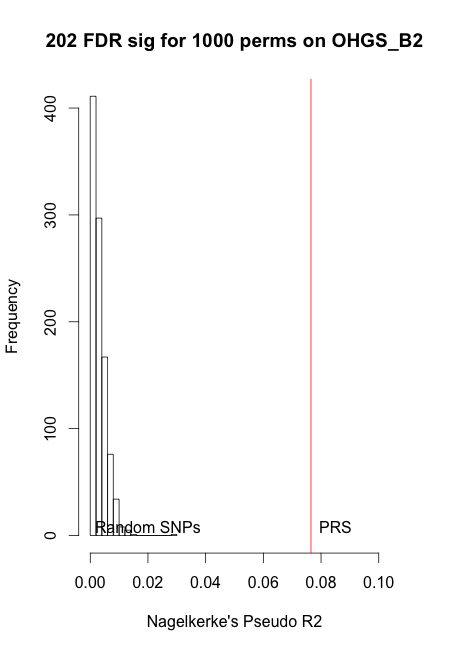
\includegraphics[width=0.5\textwidth]{Figures/b2.png}
\label{b2_perm}
\caption[$\hat{S}_{TRS}$ predicts \ac{CAD} significantly better than 1000 \ac{PRS} constructed with an equal number of \acp{SNP}.]{\textbf{$\hat{S}_{TRS}$ predicts \ac{CAD} significantly better than 1000 \ac{PRS} constructed with an equal number of \acp{SNP}.} 202 \acp{SNP} were randomly selected from post quality control imputed \acp{SNP} and a \ac{PRS} was constructed using summary information from \cite{TheCARDIoGRAMplusC4DConsortium2015} and Nagelkerke's Pseudo $R^2$ was plotted against frequency. The red line denote the Nagelkerke's $R^2$ of the true \ac{TRS} which predicts significantly $P \approx 0$ better than the random model.}
\end{figure}

These results are in line with literature values. Those in the top quintile of the \ac{PRS} were 70\% more likely to have \ac{CAD} than not (2045 cases vs 1198 controls). Similarly, those in the bottom quintile were  5\% less likely to be diagnosed with \ac{CAD} than not (1576 cases vs 1659 controls).



\section{Cardiometabolic Risk Score}

We add in each co-morbid score in a stepwise manner. $\hat{S}_{CMB; 1}$ uses just the information available for CAD and is equivalent to the above section.  $\hat{S}_{CMB; 2}$ uses information from CAD and BMI, while $\hat{S}_{CMB; 3}$ uses CAD, BMI, and LDLc. $\hat{S}_{CMB; 4}$ uses information from CAD, BMI, LDLc, and TG, while $\hat{S}_{CMB; 5}$ uses CAD, BMI, LDLc, TG, and HDLc. Note that in this section we restrict our analysis to the \ac{OHGS} cohorts along with Cleveland Clinic due to the lack of quality in lipid data present in the other cohorts. 

The summary statistics of this analysis are presented in Table \ref{cmd-sum}. Higher genetic risk scores were uniformly and significantly ($P < 2.2 \times 10^{-16}$) associated with increased risk of \ac{CAD}.

\begin{table}[H]
\centering
\begin{tabular}{lllllll}
\hline
Score & Cohort           & OR        & SE       & R2         & AIC      & AUC       \\ \hline
$\hat{S}_{CMB; 1}$     & OHGS A2          & 310.49752 & 34.52749 & 0.07650691 & 2558.277 & 0.6391285 \\
      & OHGS B2          & 259.59352 & 24.94511 & 0.07425403 & 3681.768 & 0.6339916 \\
      & OHGS C2          & 276.96733 & 45.92012 & 0.05491302 & 1318.919 & 0.6193695 \\
      & Cleveland Clinic & 153.89908 & 36.42776 & 0.01621871 & 1877.724 & 0.5740551 \\ \hline
$\hat{S}_{CMB; 2}$     & OHGS\_A2         & 252.9639  & 25.29332 & 0.09108544 & 2547.617 & 0.6555183 \\
      & OHGS\_B2         & 267.348   & 22.48745 & 0.09187763 & 3654.756 & 0.6501946 \\
      & OHGS\_C2         & 280.9237  & 38.98146 & 0.07687197 & 1300.585 & 0.6455279 \\
      & Cleveland        & 337.3714  & 35.18263 & 0.08387982 & 1791.596 & 0.6659644 \\ \hline
$\hat{S}_{CMB; 3}$     & OHGS\_A2         & 236.0145  & 26.17239 & 0.07656732 & 2570.063 & 0.6429851 \\
      & OHGS\_B2         & 255.7401  & 24.09888 & 0.0767165  & 3688.513 & 0.6371506 \\
      & OHGS\_C2         & 284.9796  & 41.16138 & 0.07121422 & 1305.337 & 0.640201  \\
      & Cleveland        & 344.9182  & 37.87978 & 0.07572764 & 1802.024 & 0.6546671 \\ \hline
$\hat{S}_{CMB; 4}$     & OHGS\_A2         & 266.5048  & 29.24856 & 0.07786803 & 2568.062 & 0.6442205 \\
      & OHGS\_B2         & 270.8893  & 26.45495 & 0.07264458 & 3697.51  & 0.6330786 \\
      & OHGS\_C2         & 298.9828  & 44.83843 & 0.06638254 & 1309.38  & 0.6337181 \\
      & Cleveland        & 372.189   & 41.80231 & 0.07218274 & 1806.542 & 0.6509422 \\ \hline
$\hat{S}_{CMB; 5}$     & OHGS\_A2         & 297.0165  & 34.10419 & 0.07234597 & 2576.54  & 0.6401786 \\
      & OHGS\_B2         & 299.0699  & 30.76742 & 0.06720315 & 3709.488 & 0.6280858 \\
      & OHGS\_C2         & 323.9172  & 50.90267 & 0.06088933 & 1313.958 & 0.6275034 \\
      & Cleveland        & 410.9963  & 48.57387 & 0.06493754 & 1815.742 & 0.6436849 \\ \hline
\end{tabular}
\label{cmd-sum}
\caption[Summary statistics from Logistic association model for $\hat{S}_{CMD}$.]{\textbf{Summary statistics from Logistic association model.} $\hat{S}_{CMD; x}$ along with the first two principal components to adjust for population stratification were used to predict \ac{CAD}. OR corresponds to the odds ratio of $\hat{S}_{TRS}$ along with its standard error (SE). $R^2$ corresponds to NagelKerke's Pseudo-$R^2$, while AIC corresponds to Akaike Information Criterion, a measure of model fit. AUC corresponds to the area under the \ac{ROC} curve as derived in the pROC package in R.}
\end{table}

In permutation analyses, each of the scores performed significantly better than an equivalent number of randomly selected \acp{SNP} in 1000 bootstraps. The random effects meta analysis \ac{AUC} values were $0.65 [ 0.64, 0.67], 0.64[0.63, 0.66], 0.64[0.63, 0.65], 0.63[0.62, 0.65]$ for scores 1 through 5 respectively. Interestingly, the more \acp{SNP} added in, the worse the model was at predicting the phenotype. The \ac{AIC} is also uniformly smaller in score 2 than in subsequent scores, meaning that this model fit the data the best. Persons in the upper quintile of this score were 81\% more likely (1725 cases vs 953 controls) to have \ac{CAD} than not (compared to 70 \% for the previous score) and people in the bottom quintile were 15.7\% less likely (1240 cases vs 1471 controls) to have \ac{CAD} than having it. There was also a substantive increase in NagelKerke's Pseudo $R^2$ in the second score compared to any other, especially in the Cleveland cohort. 

The score maintained its significance even after inclusion of biologically relevant covariates such as gender and smoking status. Additionally, the predictive accuracy of the score increased substantially after the inclusion of these covariates. After inclusion of individual's sex, a known cardiovascular risk factor, predictive accuracy increased substantially. The random effects meta analysis \ac{AUC} values were increased to $0.69[0.62, 0.76], 0.74[0.67, 0.81], 0.73 [0.66, 0.81], 0.73[0.66, 0.81], 0.73[0.66, 0.80]$ for $\hat{S}_{CMB; 1}$ through $\hat{S}_{CMB; 5}$ respectively. Again it appears as though $\hat{S}_{CMB; 2}$ is the best predictive model.


We additionally investigated whether sex significantly modulates the effect of  $\hat{S}_{CMB; .}$ and found no significant interactions. 

\subsection{Optimal Cardiometabolic Risk Score}

When optimal scores were derived, the thresholds described in Table \ref{oprs} were observed.

\begin{table}[H]
\centering

\begin{tabular}{lllll}
\hline
                  & \textbf{LDLc} & \textbf{HDLc} & \textbf{TG} & \textbf{BMI} \\ \hline
OHGS\_A2 & 0.0001        & 0.0055        & 0.1743      & 1            \\
OHGS\_B2 & 0.2484        & 0.0999        & 0.0002      & 1            \\
OHGS\_C2 & 0.1299        & 0.0085        & 0.1528      & 1            \\
CCGB\_2  & 0.1807        & 0.2039        & 0.004       & 1            \\ \hline
\end{tabular}

\caption[Optimal \ac{PRS} $P$-value thresholds.]{\textbf{Optimal \ac{PRS} $P$ value thresholds ($T_o$) derived for each trait in each cohort.} 2500 thresholds were created between $P = 0.0001$ and $P = 0.25$ and used as inclusion threshold $T$ for \ac{PRS}. These \acp{SNP} were used to construct a \ac{PRS}, which was used alongside the first two principal components and sex as covariates to predict \ac{CAD}. Their respective $P$-values of association were recorded and the maximal $-\log_{10} P$-value of association was used as the optimal threshold $T_0$.}
\label{oprs}
\end{table}


The optimal $P$ value cutoff threshold $T_o$ for \ac{BMI} was found to be $1$ for all cases as demonstrated in \ref{oprs_bmi}. We discuss this result further below, however, for now we exclude \ac{BMI} from the analysis of optimal risk scores, and opt to use just scores for the lipid traits.

\begin{figure}[H]
\centering
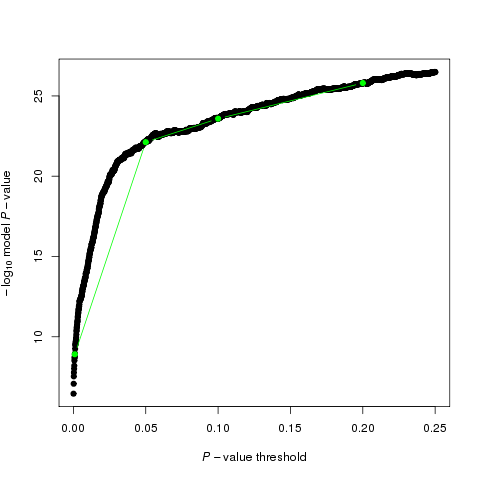
\includegraphics[width=0.5\textwidth]{Figures/PRSice_HIGH-RES_PLOT_2016-04-23.png}
\label{oprs_bmi}
\caption[Optimal $P$-value inclusion threshold for \ac{BMI}.]{\textbf{High definition assocaition plot for \ac{BMI} \acp{SNP} with \ac{CAD}.}2500 thresholds were created between $P = 0.0001$ and $P = 0.25$ and used as inclusion threshold $T$ for \ac{PRS}. These \acp{SNP} were used to construct a \ac{PRS}, which was used alongside the first two principal components and sex as covariates to predict \ac{CAD}. Their respective $P$-values of association were recorded and the maximal $-\log_{10} P$-value of association was used as the optimal threshold $T_0$. There was no maximal $-\log_{10} P$ value threshold less than 0.25, consistent with the model shown in figure \ref{pi0} with low $\pi_0$, or proportion of truly null \acp{SNP}.}
\end{figure}

Constructing a logistic regression model, we find that our cumulative score (combining optimal scores from all three traits) is significantly ($P < 2.2 \times 10^{-16}$.) associated with \ac{CAD} status, and those who have a higher \ac{PRS} tend to have higher risk for \ac{CAD}. We detail summary statistics for this association in table \ref{oprs_ss}. 



\begin{table}[H]
\centering

\begin{tabular}{lllllll}
\hline
Study & $n_{SNPs}$ & OR         & SE      & $R^2$     & AIC     & ROC    \\ \hline
OHGS\_A2 & 439971 & $2.2\times10^4$  & $1.3\times10^3$ & 0.2451 & 2313    & 0.7478 \\
OHGS\_B2 & 790128 & $3.42\times10^4$ & $1.5\times10^3$ & 0.3377 & 3061.9  & 0.7963 \\
OHGS\_C2 & 622050 & $3.34\times10^4$ & $2.5\times10^3$ & 0.3009 & 1095.1  & 0.7929 \\
CCGB\_2 & 847335 & $3.78\times10^4$ & $2.3\times10^3$ & 0.2836 & 1517.21 & 0.7953 \\ \hline
\end{tabular}
\label{oprs_ss}
\caption[Summary statistics from Logistic association model for $\hat{S}_{oCMD}$.]{\textbf{Summary statistics from Logistic association model.} $\hat{S}_{oCMD}$ along with the first two principal components to adjust for population stratification were used to predict \ac{CAD}. OR corresponds to the odds ratio of $\hat{S}_{TRS}$ along with its standard error (SE). $R^2$ corresponds to NagelKerke's Pseudo-$R^2$, while AIC corresponds to Akaike Information Criterion, a measure of model fit. AUC corresponds to the area under the \ac{ROC} curve as derived in the pROC package in R.}
\end{table}

The \ac{oPRS}, comprising optimal scores for \ac{LDLc}, \ac{HDLc}, and \ac{TG} predicts \ac{CAD} with a very high accuracy, explaining between 24.5 and 33.8 percent of variance in \ac{CAD}. The random effects meta analysis of \ac{AUC} of the \ac{ROC} curve reveals an overall \ac{AUC} of $0.78 [0.75, 0.81]$, an extremely high value (Figure \ref{oprs_meta}). 

\begin{figure}[H]
\label{oprs_meta}
\caption{Random effects meta analysis of \ac{oPRS} predicting risk for \ac{CAD}}
\centering
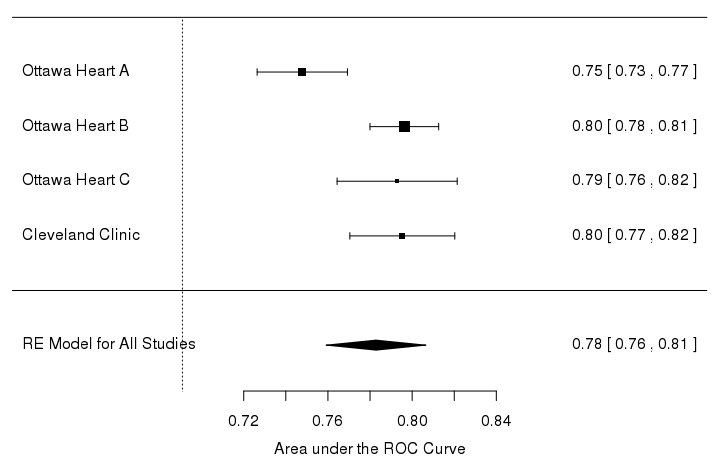
\includegraphics[width=0.5\textwidth]{Figures/oprs_meta.png}
\end{figure}


Though the \ac{AUC} varies significantly between the cohorts, it is significantly higher than any observed in either the \ac{TRS} or the \ac{CMB} scores. However, as noted in table \ref{oprs_ss}, each \ac{oPRS} comprises several hundred thousand \acp{SNP}, and it is difficult to assess whether the increase in predictive accuracy is simply a consequence of increasing the number of \acp{SNP} used to predict the phenotype, or whether it is a true biological occurrence. When an equal number of \acp{SNP} were selected at random in 1000 bootstraps, it was found that the $R^2$ of our \ac{oPRS} was not significantly $P > 0.05$ different than that obtained through permutation.


\subsection{Model Comparisons}

When the cardiometabolic $\hat{S}_{CMB; 2}$, determined to be the best predictive candidate score for \ac{CAD} was compared against the \ac{TRS} score in 1000 random bootstraps in all cohorts combined, it was found to have a significantly larger \ac{AUC} ($P < 2.2 \times 10^{-16}$). A similar result was found when the \ac{oPRS} was compared to both the \ac{TRS} and the \ac{CMB} scores.